%%%%%%%%%% doing (definition)
\def\doing{выполняем следующую последовательность действий}

%%%%%%%% 2
\section{Выполнение работы}

%%%%%%%%%%% 2.1
\subsection{Настройка FC SAN}

Запускаем симулятор Unisphere VNXe Demo.

%%%%%%%%%%%%%% 2.1.1
\subsubsection{Определение мировых имён портов хранения и сведение их в
    таблицу}

Для определения мировых имён портов хранения \doing:

\begin{enumerate_num}
    \item Переходим на вкладку <<VNXe > Settings > More configuration > Port
    Settings>>.
    \item Раскрываем модуль ввода/вывода 0 и выбираем каждый оптоволоконный
    канал для определения мирового имени и другой информации для каждого из
    портов
    хранения.
    \item Находим номер похожий на 50:06:01:60:88:Е0:02:22:50:06:01:64:08:
    Е0:02:22, где первые 16 цифр -- это мировое имя узла, а вторые 16 --
    мировое
    имя порта.
\end{enumerate_num}

\begin{figure}[ht]
    %%%%%% 2.1 (figure)
    \begin{minipage}[b]{0.5\textwidth}
        \centering
\includegraphics[width=\textwidth]{1/1.png}
        \caption{Информация о порте хранения 0 модуля I/O 0 FC}
    \end{minipage}
    %%%%%% 2.2 (figure)
    \begin{minipage}[b]{0.5\textwidth}
        \centering
\includegraphics[width=\textwidth]{1/2.png}
        \caption{Информация о порте хранения 1 модуля I/O 0 FC}
    \end{minipage}
\end{figure}
\begin{figure}[ht]
    %%%%%% 2.3 (figure)
    \begin{minipage}[b]{0.5\textwidth}
        \centering
\includegraphics[width=\textwidth]{1/3.png}
        \caption{Информация о порте хранения 2 модуля I/O 0 FC}
    \end{minipage}
    %%%%%% 2.4 (figure)
    \begin{minipage}[b]{0.5\textwidth}
        \centering
\includegraphics[width=\textwidth]{1/4.png}
        \caption{Информация о порте хранения 3 модуля I/O 0 FC}
    \end{minipage}
\end{figure}

Мировое имя и другая информация для каждого из портов хранения представлены на
рисунках 2.1, 2.2, 2.3 и 2.4. Замечаем, что для всем мировым именам порта
соответствует мировое имя узла 50:06:01:60:88:E0:02:22.

%%%%%% 2.1 (table)
\begin{table}[ht]
    \caption{Мировые имена портов хранения}
    \begin{tabular} {|c|l|l|l|}\cline{1-3}
        № & World Wide Port Name    & World Wide Node Name    \\\cline{1-3}
        1 & 50:06:01:64:08:E0:02:22 & 50:06:01:60:88:E0:02:22 \\\cline{1-3}
        2 & 50:06:01:6C:08:E0:02:22 & 50:06:01:60:88:E0:02:22 \\\cline{1-3}
        3 & 50:06:01:65:08:E0:02:22 & 50:06:01:60:88:E0:02:22 \\\cline{1-3}
        4 & 50:06:01:6D:08:E0:02:22 & 50:06:01:60:88:E0:02:22 \\\cline{1-3}
        5 & 50:06:01:66:08:E0:02:22 & 50:06:01:60:88:E0:02:22 \\\cline{1-3}
        6 & 50:06:01:6E:08:E0:02:22 & 50:06:01:60:88:E0:02:22 \\\cline{1-3}
        7 & 50:06:01:67:08:E0:02:22 & 50:06:01:60:88:E0:02:22 \\\cline{1-3}
        8 & 50:06:01:6F:08:E0:02:22 & 50:06:01:60:88:E0:02:22 \\\cline{1-3}
    \end{tabular}
\end{table}

Заполняем таблицу 2.1, используя полученную информацию.

%%%%%%%%%%%%%% 2.1.2
\subsubsection{Определение мировых имён портов хоста-инициатора и сравнение
    полученных результатов}

Для определения мировых имён портов хоста-инициатора \doing:

%%%%%% 2.5 (figure)
\begin{figure}[ht]
    \centering
\includegraphics[width=0.85\textwidth]{1/5.png}
    \caption{Вкладка <<VNXe > Hosts > Initiators>>}
\end{figure}

\begin{enumerate_num}
    \item Переходим на вкладку <<VNXe > Hosts > Initiators>>.
    \item Находим номер похожий на 10:00:00:90:FA:14:3D:60:20:00:00:90:FA:
    14:3D:60, где первые 16 цифр -- это мировое имя порта хоста-инициатора.
\end{enumerate_num}

Сравниваем занесенную в таблицу 2.1 информацию с выводом конфигурации Fibre
Channel свитча отображенную в конце данного файла (рисунок 2.5). В результате
сравнения делаем вывод о том, что отображение имён на рисунке не совпадает с
таблицей.

%%%%%%%%%%%%%% 2.1.3
\subsubsection{Предложение изменений, которые, возможно, необходимо внести в
    конфигурацию}

Основываясь на наших исследованиях, мы можем предложить изменение, которые
нужно внести в конфигурацию: изменить формат вывода мирового имени инициаторов.

%%%%%%%%%%% 2.2
\subsection{Установка используемого ПО}

Для выполнения лабораторной работы требуется установить Wireshark. Поскольку
работа подразумевает использования снятых дампов трафика, программу можно
установить на хостовой операционной системе. Для этого выполняем следующую
команду:

\begin{lstlisting}
sudo nala install wireshark
\end{lstlisting}

Результат выполнения этой команды представлен на рисунке 2.6.

\begin{figure}[ht]
    \centering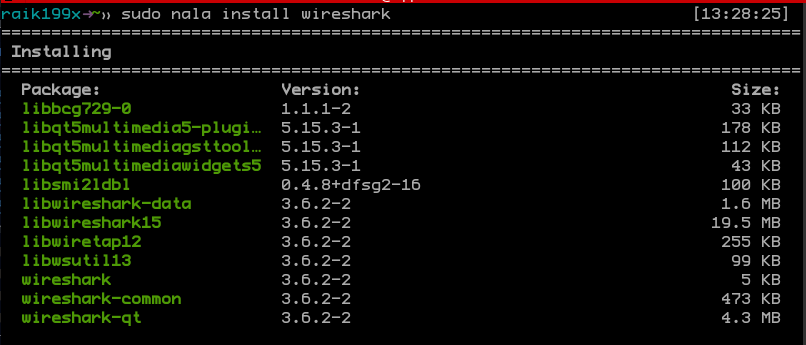
\includegraphics[width=1\textwidth]{1/6.png}
    \caption{Установка программы-анализатора трафика wireshark}
\end{figure}

После завершения данной операции, мы переходим к важному этапу - анализу дампа
трафика. Этот процесс позволяет нам более детально изучить передачу данных.

Анализ дампа трафика помогает нам лучше понять, как данные передаются и
взаимодействуют между сетевыми узлами.

%%%%%%%%%%% 2.3
\subsection{Исследование FC SAN Trace}

Запускаем программу-анализатор трафика Wireshark. В ней же открываем файл
<<FC\_SAN\_Trace.pcap>>.

%%%%%%%%%%%%%% 2.3.1
\subsubsection{Ответ на вопрос <<Что такое FLOGI?>>}

FLOGI (Fabric Login) является процессом аутентификации и инициализации
устройства Fibre Channel в хранилищных сетях.

В процессе FLOGI устройство Fibre Channel инициирует соединение с коммутатором
или шлюзом Fibre Channel в сети. Во время этого процесса устройство отправляет
запрос на вход в сеть, который включает в себя его идентификатор и другую
информацию. Коммутатор или шлюз проверяют запрос и, если он успешен,
предоставляют устройству доступ к Fibre Channel сети.

FLOGI выполняется на уровне волоконного канала (FC) и является первым шагом в
установлении соединения между устройством и сетью Fibre Channel. После
успешного выполнения FLOGI устройство может выполнять другие операции, такие
как регистрация в зоне (зонирование), обмен данными и управление блокировками в
сети Fibre Channel.

%%%%%%%%%%%%%% 2.3.2
\subsubsection{Ответ на вопрос <<Какое мировое имя у первого порта
    принадлежащего Fibre Channel Fabric?>>}

Для того, чтобы дать ответ на данный вопрос \doing:

%%%%%% 2.7 (figure)
\begin{figure}[ht]
    \centering
\includegraphics[width=1\textwidth]{4/7.png}
    \caption{Wireshark. Поиск мирового имени первого порта принадлежащего Fibre
        Channel Fabric}
\end{figure}

\begin{enumerate_num}
    \item Прописываем <<fc>> в фильтре и нажимаем на кнопку <<Apply>>.
    \item Ищем кадры протокола FC ELS (Exchange Link Services).
    \item Из найденных кадров выбираем первый, у которого в поле <<Info>>
    указано <<PLOGI>> (Port Login). Раскрываем секцию <<FC ELS>>.
    \item Раскрываем подсекцию <<Common Svc Parameters>>.
    \item Находим поля <<N\_Port Port\_Name>> (мировое имя порта) и
    <<Fabric/Node Name>> (мировое имя устройства).
    \item Ответом является значение в поле <<N\_Port Port\_Name>>.
\end{enumerate_num}

Результат выполнения вышеперечисленных шагов представлен на рисунке 2.7.

Ответ: 10:00:00:00:c9:44:49:55 (Emulex).

%%%%%%%%%%%%%% 2.3.3
\subsubsection{Ответ на вопрос <<Почему поле идентификатора источника (S\_ID)
    кадра FLOGI содержит одни нули?>>}

В процессе FLOGI, когда устройство Fibre Channel инициирует вход в сеть, оно
отправляет кадр FLOGI для запроса адреса. При этом поле S\_ID, которое обычно
содержит идентификатор порта источника, устанавливается в нулевое значение
(0x0000). Это сигнализирует коммутатору Fibre Channel о необходимости выделить
новый адрес порта для устройства.

%%%%%% 2.8 (figure)
\begin{figure}[ht]
    \centering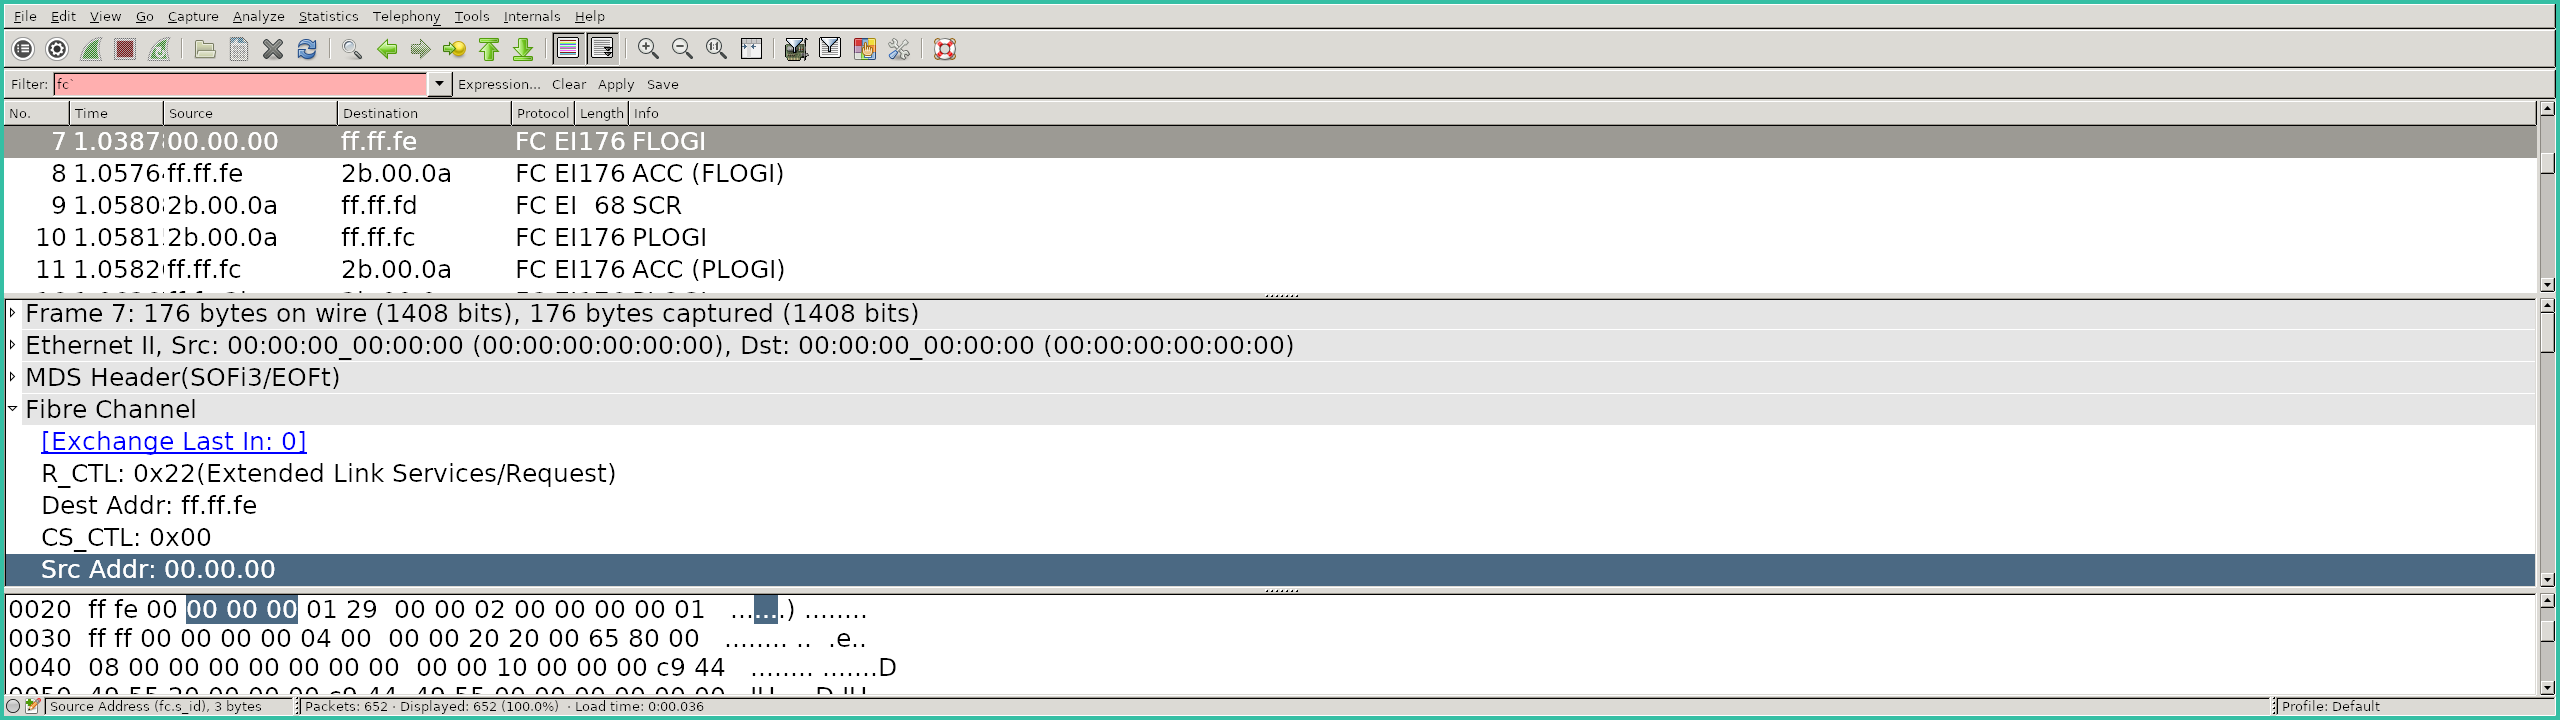
\includegraphics[width=1\textwidth]{4/8.png}
    \caption{Wireshark. Поле идентификатора источника кадра FLOGI}
\end{figure}

На рисунке 2.8 можно заметить, что это действительно так.

%%%%%%%%%%%%%% 2.3.4
\subsubsection{Ответ на вопрос <<Какой адрес назначен первому порту
    принадлежащему Fibre Channel Fabric?>>}

Для того, чтобы дать ответ на данный вопрос \doing:

%%%%%% 2.9 (figure)
\begin{figure}[ht]
    \centering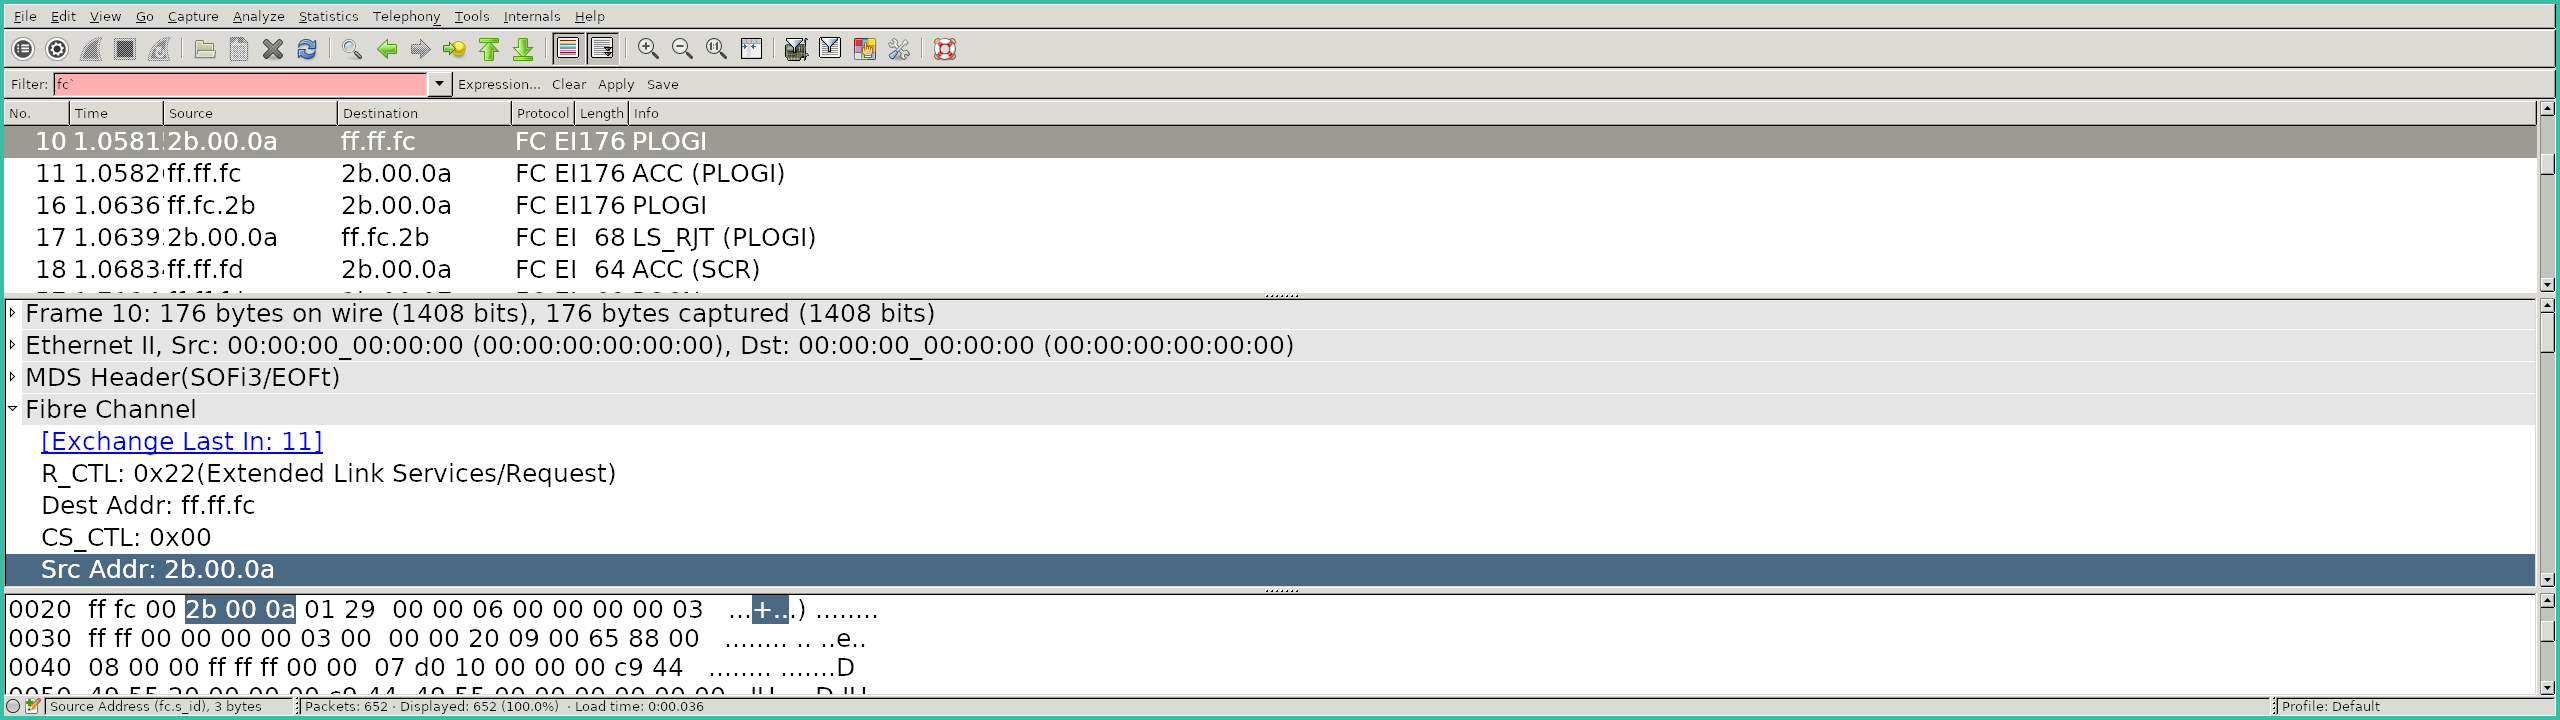
\includegraphics[width=1\textwidth]{4/9.png}
    \caption{Wireshark. Поиск адреса, назначенного первому порту принадлежащему
        Fibre Channel Fabric}
\end{figure}

\begin{enumerate_num}
    \item Прописываем <<fc>> в фильтре и нажимаем на кнопку <<Apply>>.
    \item Ищем кадры протокола FC ELS (Exchange Link Services).
    \item Из найденных кадров выбираем первый, у которого в поле <<Info>>
    указано <<PLOGI>> (Port Login).
    \item Раскрываем секцию <<Fibre Channel>>.
    \item Находим поля <<Dest Addr>> (поле идентификатора назначения) и <<Src
    Addr>> (поле идентификатора источника).
    \item Ответом является значение поля <<Src Addr>>.
\end{enumerate_num}

Результат выполнения вышеперечисленных шагов представлен на рисунке 2.9.

Ответ: 2b.00.0a.

%%%%%%%%%%%%%% 2.3.5
\subsubsection{Ответ на вопрос <<Какое шестнадцатеричное представление FC-4
    TYPE запрашивается для заданного кадра и какой протокол оно
    представляет?>>}

Под заданным кадром подразумевается один из кадров, посланных узлом (Fibre
Channel Fabric), который отмечен как GID\_FT (Get Port IDs -- FC-4 Type).

%%%%%% 2.10
\begin{figure}[ht]
    \centering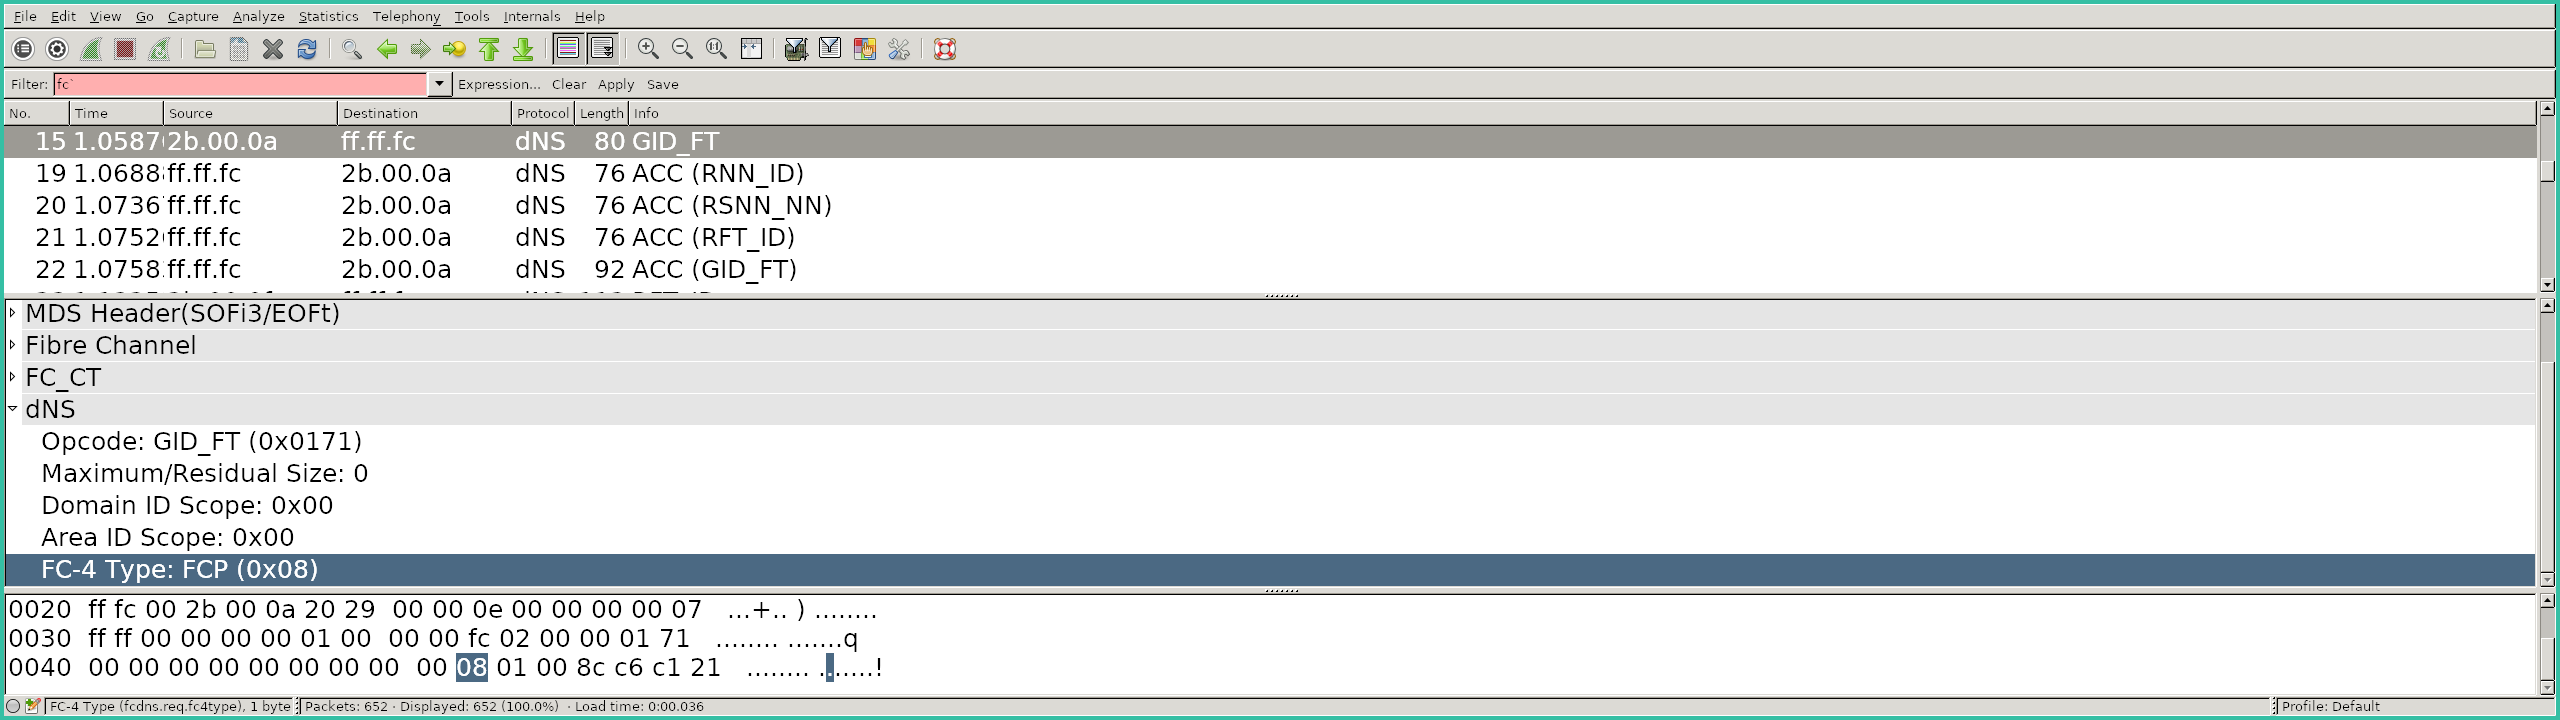
\includegraphics[width=1\textwidth]{4/10.png}
    \caption{Wireshark. Поле <<FC-4 TYPE>> кадра <<GID\_FT>>}
\end{figure}

Как следует из содержимого заданного кадра (рисунок 2.10), запрашивается
шестнадцатеричное представление FC-4 TYPE 0x08, которое представляет протокол
SCSI\_FCP (SCSI Fibre Channel Protocol).

Ответ: 0x08, SCSI\_FCP.

%%%%%%%%%%%%%% 2.3.6
\subsubsection{Ответ на вопрос <<Какой сервис ответственен за GID\_FT (Get Port
    IDs) запрос?>>}

Сервис <<Name Server>> ответственен за обработку GID\_FT запросов и
предоставление информации о доступных портах в сети Fibre Channel.

Ответ: Name Server.
